% -*- mode: fundamental -*-

% ****************************************************************

\chapter{BSV: Rules and Methods II: Improved performance with Concurrent Registers}

\markboth{Ch \arabic{chapter}: BSV: Rules II}{\copyrightnotice}

\setcounter{page}{1}
% \renewcommand{\thepage}{\arabic{page}}
\renewcommand{\thepage}{\arabic{chapter}-\arabic{page}}

\label{ch_Rules_II}

% ****************************************************************

\section{Introduction}

In Section~\ref{Sec_Constraints_on_Mapping_Rules_to_a_Clock} we
discussed constraints on mapping rules into clocked digital hardware.
In particular, executing two rules on the same clock edge may result
in an ordering conflict, and therefore the compiler produces a Rule
Controller to suppress simultaneous firing.  This has some
consequences on the performance of BSV programs, depending on the
primitive modules they use.  We illustrate this problem in
Section~\ref{Sec_Up_Down_Counter}, and then show a general-purpose
solution in Section~\ref{Sec_CRegs} using ``\emph{Concurrent
Registers}'' (or \verb|CReg|s).

Finally, in Section~\ref{Sec_RWires} we show an older solution called
\verb|RWire|s.  We deprecate use of \verb|RWire|s in favor of
\verb|CReg|s, but they are still supported by the compiler (Drum and
Fife codes do not use any \verb|RWire|s).

% ****************************************************************

\section{Example: Counter with {\tt .incr} and {\tt .decr} methods}

\label{Sec_Up_Down_Counter}

Consider the following ``Up-Down Counter'' module interface:

{\small
\begin{Verbatim}[frame=single, numbers=left]
interface Up_Down_Counter_IFC;
   method Action   incr;
   method Action   decr;
   method Bit #(4) val;
endinterface
\end{Verbatim}
}

The specification for any module implementing this is this:
internally, the module should contain a register that can hold values
in the range 0..15, and, the methods do the following:

\begin{tightlist}
 \item \verb|incr|  increments the counter if it is $< 15$
 \item \verb|decr|  decrements the counter if it is $> 0$
 \item \verb|val|   returns the current value of the counter
\end{tightlist}

Up-down counters are often used for ``credit-based flow control''.
For example, a networking application may send network packets and,
concurrently, receive acknowledgments for previously sent packets, but
the network may not accommodate more than 15 such packets.  Suppose
the register is initialized to 15.  This represents the number of
available ``credits'', {\ie} the number of packets that can be sent
without acknowledgement.  We decrement it whenever a packet is sent,
and increment it whenever an acknowlegement is received.  Thus, it
prevents us from sending more than 15 packets without acknowlegement.

Here is a proposed module to implement the interface:

{\small
\begin{Verbatim}[frame=single, numbers=left]
module mkUp_Down_Counter_I (Up_Down_Counter_IFC);
   // STATE
   Reg #(Bit #(4)) rg_counter <- mkReg (15);

   // ----------------------------------------------------------------
   // INTERFACE
   method Action incr (rg_counter != 15);
      rg_counter <= rg_counter + 1;
   endmethod

   method Action decr; (rg_counter != 0);
      rg_counter <= rg_counter - 1;
   endmethod

   method Bit #(4) val;
      return rg_counter;
   endmethod
endmodule
\end{Verbatim}
}

% ================================================================

\subsection{Semantic and Performance Analysis of {\tt
            mkUp\_Down\_Counter\_I} when mapped to clocked hardware}

Suppose we have three rules, each invoking one of the three methods on
the same module.  Which pairs of rules can fire on the same clock?

\begin{itemize}

 \item \verb|val| \emph{and} \verb|incr|?

       Yes: Clocked execution is consistent with rule-at-a-time
       semantics where the rule with \verb|val| fires before the rule
       with \verb|incr|.  (And similary, a rule invoking \verb|val|
       can fire on the same clock as a rule invoking \verb|decr|.)

 \item \verb|incr| \emph{and} \verb|decr|?

       No, for both reasons discussed in
       Section~\ref{Sec_Constraints_on_Mapping_Rules_to_a_Clock}.
       There would be an action/resource conflict because both rules
       cannot write the same register at the same instant.  There
       would be an ordering confict because rule-at-a-time semantics
       demands that one rule's update is visible to the other (in
       whichever order they may fire).

\end{itemize}

The key takeaway is that \verb|incr| and \verb|decr| cannot be invoked
on the same clock (same instant).  To revisit our credit-based
flow-control example: on each clock we can either send a packet or
receive an acknowledgement, but not both.

% ****************************************************************

\section{Concurrent Registers {\tt CReg}s, and a Faster Up-Down Counter}

\label{Sec_CRegs}

A Concurrent Register, or \verb|CReg|, is a module provided by the
\emph{bsc} library.  This is an excerpt from the library documentation:

{\small
\begin{Verbatim}[frame=single, numbers=left]
module mkCReg #(parameter Integer n,
                parameter a_type resetval)
              (Reg#(a_type) ifc[])
\end{Verbatim}
}

The interface is an \emph{array} of register interfaces, indicated by
the square brackets.  A \verb|CReg| module is instantiated with syntax
like this:

{\small
\begin{Verbatim}[frame=single, numbers=left]
   // parameter n is 2, resetval is 15
   Array #(Reg #(Bit #(4))) crg_counter <- mkCReg (2, 15);
\end{Verbatim}
}

This instantiates a \verb|CReg| whose interface is an array of 2
register interfaces, and whose reset value is 15.  Each interface can
be accessed by indexing: {\tt crg\_counter~[0]} and {\tt
crg\_counter~[1]}.

The key properties of a \verb|CReg| \verb|x| with an array of \verb|n|
register interfaces is:

\begin{itemize}
 \item All the methods can be invoked in the same clock.

 \item A read at the $j$'th register interface,{\ie} {\tt x[$j$].\_read}
       returns the latest of:

       \begin{tightlist}
        \item the value in the register;
        \item if {\tt x[0].\_write($v_0$)} is being invoked, the value $v_0$;
        \item if {\tt x[1].\_write($v_1$)} is being invoked, the value $v_1$;
        \item ...
        \item if {\tt x[$j-1$].\_write($v_{n-1}$)} is being invoked, the value $v_{n-1}$;
       \end{tightlist}

 \item The register value is updated with the latest of:

       \begin{tightlist}
        \item the current value in the register;
        \item if {\tt x[0].\_write($v_0$)} is being invoked, the value $v_0$;
        \item if {\tt x[1].\_write($v_1$)} is being invoked, the value $v_1$;
        \item ...
        \item if {\tt x[$n-1$].\_write($v_{n-1}$)} is being invoked, the value $v_{n-1}$;
       \end{tightlist}
\end{itemize}

% ================================================================

\subsection{A possible hardware implementation of a CReg}

\label{Sec_CReg_HW}

Figure~\ref{Fig_CReg_HW} shows a possible hardware implementation of a CReg.
\begin{figure}[htbp]
  \centerline{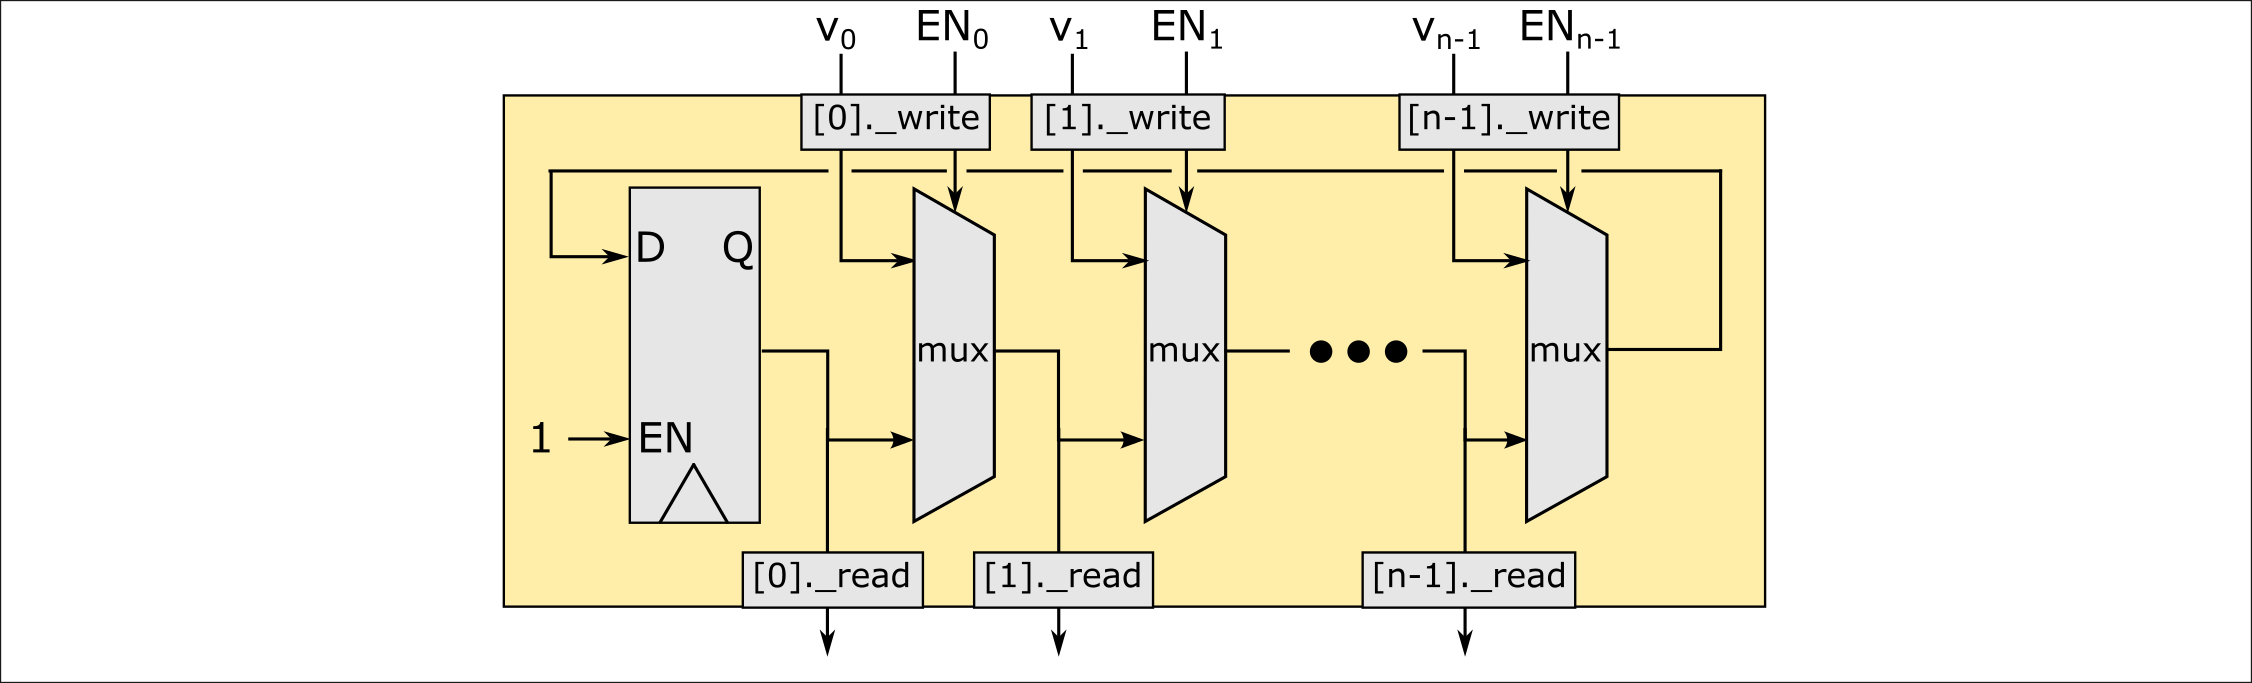
\includegraphics[width=6in,angle=0]{Figures/Fig_CReg_HW}}
  \caption{\label{Fig_CReg_HW} A possible hardware implementation of a CReg}
\end{figure}
On the left is a regular D flip flop.  To its right is a combinational
circuit comprised of a series of $n$ multiplexers, where $n$ is the
interface array size for the CReg.  The top and bottom depict the $n$
\verb|.write| and \verb|.read| methods, respectively.

The $j^{th}$ multiplexer selects either the output of the previous
element (D flip flop or multiplexer), or the data argument of the {\tt
[$j$].\_write} method.  The selection is controlled by the EN input of
the {\tt [$j$].\_write} method.  Thus, if the {\tt [$j$].\_write} method
is currently being invoked, that data is fed onward, otherwise the
data from the previous element.

The {\tt [$j$].\_read} method returns the value before the $j$'th
multiplexer.

A little study of the diagram will show that it indeed implements the
semantics described in the previous section.

% ================================================================

\subsection{A Faster Up-Down Counter, using a {\tt CReg}}

\label{Sec_Faster_Up_Down_Counter}

Here is an alternative module implementing our Up-Down Counter
interface, using a \verb|CReg|:

{\small
\begin{Verbatim}[frame=single, numbers=left]
module mkUp_Down_Counter_I (Up_Down_Counter_IFC);
   // STATE
   Array #(Reg #(Bit #(4))) crg_counter <- mkCReg (2,15);

   // ----------------------------------------------------------------
   // INTERFACE
   method Action incr (rg_counter != 15);
      rg_counter [0] <= rg_counter [0] + 1;
   endmethod

   method Action decr; (rg_counter != 0);
      rg_counter [1] <= rg_counter [1] - 1;
   endmethod

   method Bit #(4) val;
      return rg_counter [0];
   endmethod
endmodule
\end{Verbatim}
}

Now, three rules invoking the three methods can all be invoked on the
same clock.  Further, when they are invoked in the same clock, it
answers the question, ``What value does \verb|val| return?'':

\begin{quote}
The original value in the CReg? \\
Or the value after the increment? \\
Or the value after the decrement? \\
Or the value after the increment and decrement?
\end{quote}

Per the semantics of \verb|CReg|, it returns \verb|rg_counter[0]|,
which is the original value in the CReg.  If we were to return
\verb|rg_counter[1]|, it would return the value after the increment
and before the decrement.  If our CReg had an array of 3 register
interfaces intead of 2, we could return \verb|rg_counter[2]| which
would be the value after both the increment and decrement.

% ----------------
\hdivider

\Exercise

Consider the following module implementing a 1-element FIFO:

{\small
\begin{Verbatim}[frame=single, numbers=left]
module mkFIFO (FIFO #(Bit #(32)));
   Reg #(Bit #(32)) rg_data <- mkRegU;
   Reg #(Bool)      rg_full <- mkReg (False);

   // ----------------
   // INTERFACE

   method Bit #(32) first () if (rg_full);
      return rg_data;
   endmethod

   method Action deq () if (rg_full);
      rg_full <= False;
   endmethod

   method Action enq (Bit #(32) x) if (! rg_full);
      rg_data <= x;
      rg_full <= True;
   endmethod

   method Action clear;
      rg_full <= False;
   endmethod
endmodule
\end{Verbatim}
}

Explain why \verb|enq| and \verb|deq| cannot be invoked on the same clock.

Explain why \verb|enq| (or \verb|deq|) and \verb|clear| cannot be invoked on the same clock.

Replace either or both registers with CRegs so that \verb|enq| and
\verb|deq| can be invoked on the same clock.  Create two versions,
with these two different semantics:

\begin{itemize}

  \item It is equivalent to rule-at-a-time semantics where \verb|deq|
        happens before \verb|enq|.  Such a FIFO is called a
        ``PipelineFIFO'' because it behaves like FIFO between pipeline
        stages, where on each clock tick the downstream stage can
        consume the current FIFO contents and the upstream stage can
        produce a new value into the FIFO.  PipelineFIFOs are
        available in the \emph{bsc} library in the \verb|SpecialFIFOs|
        package.

  \item It is equivalent to rule-at-a-time semantics where \verb|enq|
        happens before \verb|deq|.  Such a FIFO is called a
        ``BypassFIFO'' because the downstream consumer can immediately
        receive a value currently being enqueued by the upstream
        producer.  BypassFIFOs are available in the \emph{bsc} library
        in the \verb|SpecialFIFOs| package.

\end{itemize}

\emph{Hint}: the two versions differ only in the CReg indexes used int
the methods.

\Endexercise
% ----------------

% ****************************************************************

\section{Alternatives to CRegs: RWires and their variants (deprecated)}

\label{Sec_RWires}

In digital hardware,

\begin{itemize}

 \item a register communicates a value across clocks (from one clock to succeeding clocks), and

 \item a wire communicates a value within a clock (from state element
       to gate, from gate to gate, and from gate to state element).

\end{itemize}

A BSV register is a standard digital hardware register.  A BSV CReg
plays the role of both register and wires, communicating values
flexibly within a clock and across clocks, depending on whether its
methods are invoked within a clock or across clocks.  The concept of
CRegs was first proposed by Daniel Rosenband and Arvind at MIT
\cite{RosenbandMEMOCODE04, Rosenband2005b} (they were originally
called ``Ephemeral History Registers'' or EHRs).

Before the invention of CRegs, BSV had a facility to manage
intra-clock communication, called the ``\verb|RWire|''.  These are
still available in BSV, along with several specializations:
``\verb|Wire|'', ``\verb|BypassWire|'', ``\verb|DWire|'', and
``\verb|PulseWire|''.  Please see the \emph{bsc} library documentation
for detailed information.

CRegs are semantically preferable to RWires because they fit cleanly
into rule-at-a-time semantics, where a CReg can be treated as an
ordinary register.  The semantics of a BSV program with CRegs can be
explained purely at the rule-at-a-time level, with no mention of
clocks.  RWires, on the other hand, are only meaninful with clocks,
and are therefore semantically messier.

Since the inclusion of CRegs into the \emph{bsc} library, the need for
\verb|RWire| and its variants has mostly disappeared.

% ****************************************************************
